
\documentclass[border=5pt]{standalone}
\usepackage{tikz}
\usetikzlibrary{arrows.meta, backgrounds, decorations.pathreplacing, fit, shapes.geometric}
\usepackage{amsmath, amssymb}
\usepackage{bm}

\definecolor{colglobal}{HTML}{4F6D7A}
\definecolor{colpop}{HTML}{8F5A83}
\definecolor{coldet}{HTML}{1F9D8A}
\definecolor{colsample}{HTML}{8A4F7D}
\definecolor{coldata}{HTML}{D8D8D8}

\tikzset{
    dag node/.style={
        draw=black!70, semithick, align=center,
        font=\scriptsize, inner sep=2.3pt,
    },
    global/.style={dag node, rectangle, rounded corners=2pt,
        minimum width=1.45cm, minimum height=0.56cm, fill=colglobal!10},
    input/.style={dag node, rectangle, rounded corners=2pt,
        dashed, draw=black!60, minimum width=1.45cm,
        minimum height=0.56cm, fill=coldata!35},
    selection/.style={dag node, rectangle, dashed, draw=black!60,
        fill=white, minimum width=1.85cm, minimum height=0.56cm},
    popdist/.style={dag node, rectangle, draw=colpop!85!black,
        dashed, fill=colpop!8, minimum height=0.66cm,
        text width=1.95cm, inner sep=1.3pt},
    latent/.style={dag node, ellipse, fill=white,
        minimum width=1.45cm, minimum height=0.58cm},
    det/.style={dag node, diamond, aspect=2.35, draw=coldet!85!black,
        fill=coldet!8, inner xsep=1pt, inner ysep=1pt},
    sample/.style={dag node, rectangle, draw=colsample!85!black,
        fill=colsample!8, minimum height=0.62cm,
        text width=1.95cm, inner sep=1.3pt},
    data/.style={dag node, rectangle, very thick, fill=coldata,
        minimum width=1.5cm, minimum height=0.56cm},
    conditioned/.style={data, double, double distance=1pt},
    plate/.style={draw=black!55, rounded corners=5pt, dashed,
        inner xsep=9pt, inner ysep=10pt},
    level label/.style={font=\scriptsize, text=black!70},
    dag edge/.style={-{Stealth[length=3pt, width=2.5pt]}, thin,
        draw=black!55},
    sel edge/.style={dag edge, draw=black!38},
}

\begin{document}
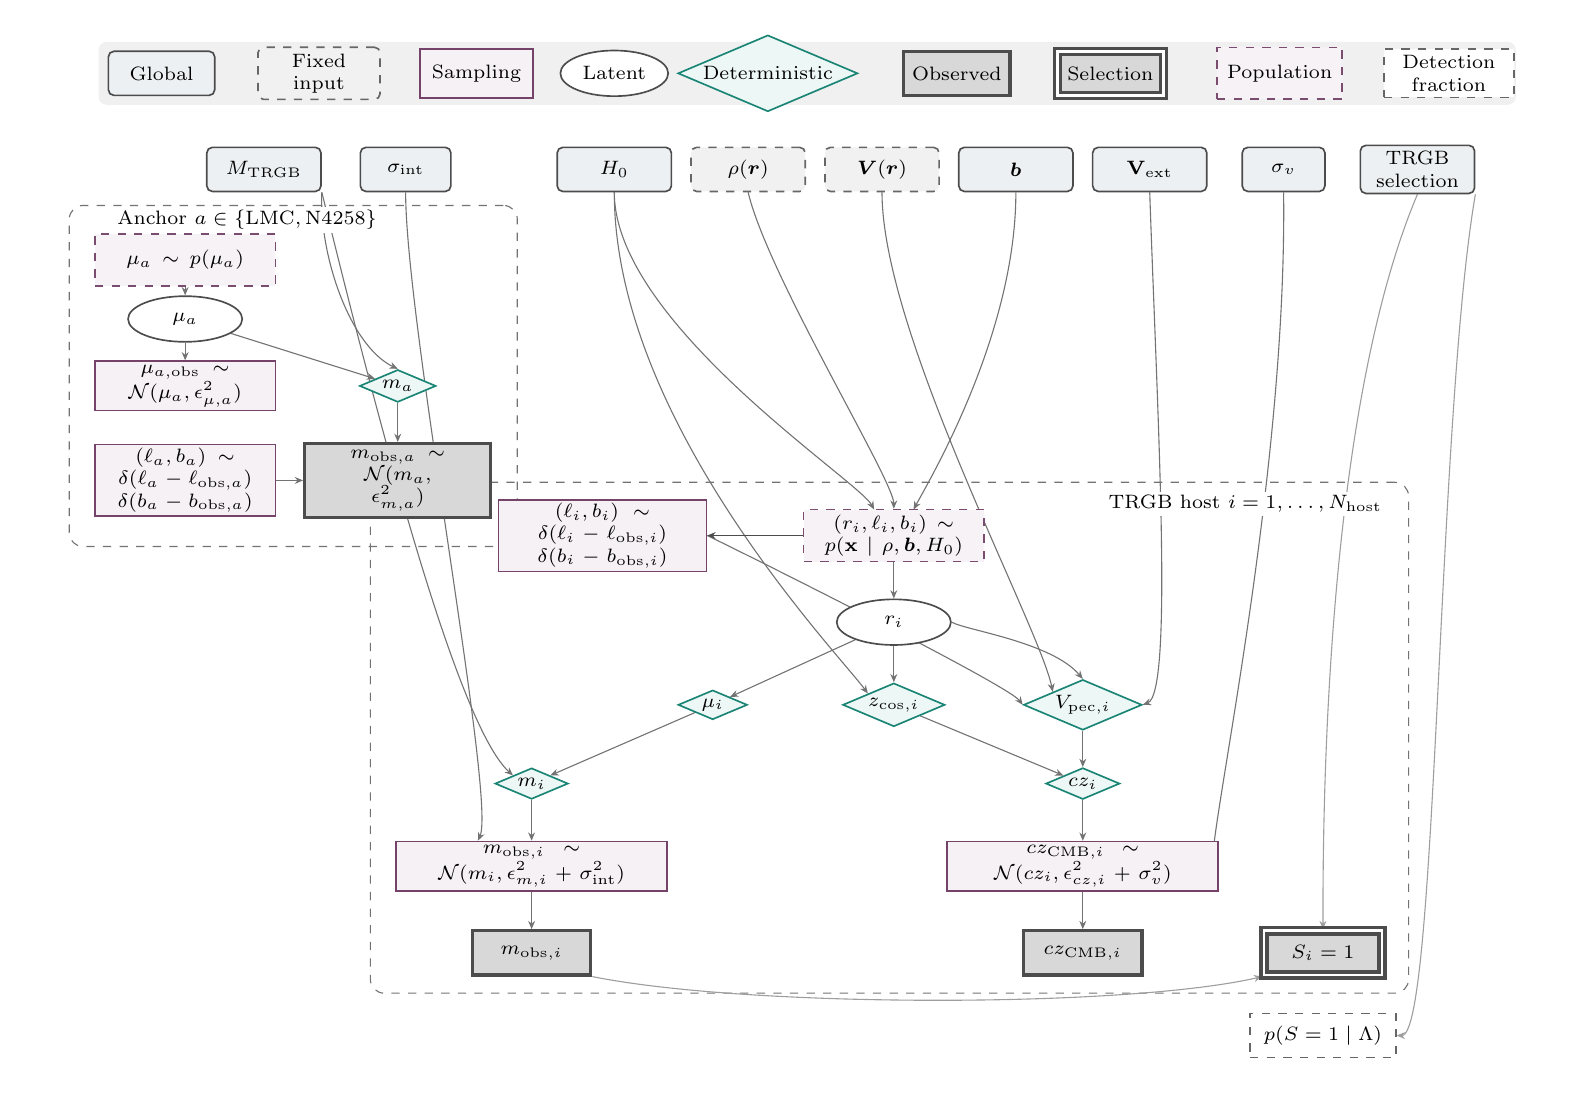
\begin{tikzpicture}

\useasboundingbox (-2.25, -3.40) rectangle (17.15, 10.00);

% ===== LEGEND =====
\begin{scope}[on background layer]
    \fill[black!6, rounded corners=3pt] (-1.35, 9.02) rectangle (16.65, 9.82);
\end{scope}
\node[global, minimum width=1.35cm] at (-0.55, 9.42) {Global};
\node[input, minimum width=1.55cm] at (1.45, 9.42) {Fixed\\input};
\node[sample, text width=1.35cm] at (3.45, 9.42) {Sampling};
\node[latent, minimum width=1.25cm] at (5.20, 9.42) {Latent};
\node[det, minimum width=1.25cm] at (7.15, 9.42) {Deterministic};
\node[data, minimum width=1.35cm] at (9.55, 9.42) {Observed};
\node[conditioned, minimum width=1.35cm] at (11.50, 9.42) {Selection};
\node[popdist, text width=1.50cm] at (13.65, 9.42) {Population};
\node[selection, minimum width=1.65cm] at (15.80, 9.42) {Detection\\fraction};

% ===== NODES =====
\node[global] (Mtrgb) at (0.75, 8.20) {$M_{\rm TRGB}$};
\node[global, minimum width=1.15cm] (sigint) at (2.55, 8.20) {$\sigma_{\rm int}$};
\node[global] (H0) at (5.20, 8.20) {$H_0$};
\node[input] (rho) at (6.90, 8.20) {$\rho(\bm{r})$};
\node[input] (Vfield) at (8.60, 8.20) {$\bm{V}(\bm{r})$};
\node[global] (bias) at (10.30, 8.20) {$\bm{b}$};
\node[global] (pv) at (12.00, 8.20) {$\mathbf{V}_{\rm ext}$};
\node[global, minimum width=1.05cm] (sigv) at (13.70, 8.20) {$\sigma_v$};
\node[global] (selcuts) at (15.40, 8.20) {TRGB\\selection};
\node[popdist, text width=2.20cm] (anchprior) at (-0.25, 7.05) {$\mu_a \sim p(\mu_a)$};
\node[latent] (anchmu) at (-0.25, 6.30) {$\mu_a$};
\node[sample, text width=2.20cm] (anchgeom) at (-0.25, 5.45) {$\mu_{a,\rm obs} \sim$\\$\mathcal{N}(\mu_a,\epsilon_{\mu,a}^2)$};
\node[det] (anchmtrue) at (2.45, 5.45) {$m_a$};
\node[sample, text width=2.20cm] (anchsky) at (-0.25, 4.25) {$(\ell_a,b_a) \sim$\\$\delta(\ell_a-\ell_{{\rm obs},a})$\\$\delta(b_a-b_{{\rm obs},a})$};
\node[data, text width=2.20cm] (anchmobs) at (2.45, 4.25) {$m_{{\rm obs},a} \sim$\\$\mathcal{N}(m_a,$\\$\epsilon_{m,a}^2)$};
\node[sample, text width=2.55cm] (skydelta) at (5.05, 3.55) {$(\ell_i,b_i) \sim$\\$\delta(\ell_i-\ell_{{\rm obs},i})$\\$\delta(b_i-b_{{\rm obs},i})$};
\node[popdist, text width=2.20cm] (rdist) at (8.75, 3.55) {$(r_i,\ell_i,b_i) \sim$\\$p(\mathbf{x}\mid\rho,\bm{b},H_0)$};
\node[latent] (rtrue) at (8.75, 2.45) {$r_i$};
\node[det] (mu) at (6.45, 1.40) {$\mu_i$};
\node[det] (zcos) at (8.75, 1.40) {$z_{{\rm cos},i}$};
\node[det] (vpec) at (11.15, 1.40) {$V_{{\rm pec},i}$};
\node[det] (mtrue) at (4.15, 0.40) {$m_i$};
\node[det] (cztrue) at (11.15, 0.40) {$cz_i$};
\node[sample, text width=3.35cm] (msamp) at (4.15, -0.65) {$m_{{\rm obs},i} \sim$\\$\mathcal{N}(m_i,\epsilon_{m,i}^2+\sigma_{\rm int}^2)$};
\node[sample, text width=3.35cm] (czsamp) at (11.15, -0.65) {$cz_{{\rm CMB},i} \sim$\\$\mathcal{N}(cz_i,\epsilon_{cz,i}^2+\sigma_v^2)$};
\node[data] (mobs) at (4.15, -1.75) {$m_{{\rm obs},i}$};
\node[data] (czobs) at (11.15, -1.75) {$cz_{{\rm CMB},i}$};
\node[conditioned] (selected) at (14.20, -1.75) {$S_i=1$};
\node[selection] (detfrac) at (14.20, -2.80) {$p(S=1\mid\Lambda)$};

% ===== PLATES =====
\begin{scope}[on background layer]
    \node[plate, fit=(anchprior)(anchmu)(anchgeom)(anchmtrue)(anchsky)(anchmobs)] {};
    \node[plate, inner ysep=6pt, fit=(skydelta)(rdist)(rtrue)(mu)(zcos)(vpec)(mtrue)(cztrue)(msamp)(czsamp)(mobs)(czobs)(selected)] {};
\end{scope}

% ===== EDGES =====
\begin{scope}[on background layer]
\draw[dag edge] (Mtrgb.south east) .. controls (1.45, 7.1) and (1.85, 5.95) .. (anchmtrue.north);
\draw[dag edge] (anchprior) -- (anchmu);
\draw[dag edge] (anchmu) -- (anchgeom);
\draw[dag edge] (anchmu) -- (anchmtrue);
\draw[dag edge] (anchmtrue) -- (anchmobs);
\draw[dag edge] (anchsky) -- (anchmobs);
\draw[dag edge] (rho.south) .. controls (7.15, 6.85) and (8.75, 4.25) .. (rdist.north);
\draw[dag edge] (bias.south) .. controls (10.30, 6.10) and (9.20, 4.25) .. (9.00, 3.88);
\draw[dag edge] (H0.south) .. controls (5.20, 6.25) and (8.30, 4.25) .. (8.50, 3.88);
\draw[dag edge] (rdist) -- (rtrue);
\draw[dag edge] (rtrue) -- (mu);
\draw[dag edge] (rtrue) -- (zcos);
\draw[dag edge] (H0.south) .. controls (5.20, 5.00) and (8.05, 2.05) .. (zcos.north west);
\draw[dag edge] (Vfield.south) .. controls (8.60, 6.10) and (10.6, 2.40) .. (vpec.north west);
\draw[dag edge] (pv.south) .. controls (12.10, 5.00) and (12.30, 1.55) .. (vpec.east);
\draw[dag edge] (skydelta.east) .. controls (7.0, 3.25) and (10.20, 1.65) .. (vpec.west);
\draw[dag edge] (rtrue.east) .. controls (9.65, 2.35) and (10.75, 2.20) .. (vpec.north);
\draw[dag edge] (Mtrgb.south east) .. controls (2.20, 5.00) and (3.20, 1.15) .. (mtrue.north west);
\draw[dag edge] (mu) -- (mtrue);
\draw[dag edge] (mtrue) -- (msamp);
\draw[dag edge] (sigint.south) .. controls (2.55, 6.25) and (3.70, 0.20) .. ([xshift=1.05cm]msamp.north west);
\draw[dag edge] (msamp) -- (mobs);
\draw[dag edge] (zcos) -- (cztrue);
\draw[dag edge] (vpec) -- (cztrue);
\draw[dag edge] (cztrue) -- (czsamp);
\draw[dag edge] (sigv.south) .. controls (13.75, 4.10) and (12.65, -0.65) .. (czsamp.east);
\draw[dag edge] (czsamp) -- (czobs);
\draw[sel edge] (selcuts.south) .. controls (14.2, 5.05) and (14.2, -0.20) .. (selected.north);
\draw[sel edge] (mobs.south east) .. controls (6.90, -2.45) and (11.70, -2.45) .. (selected.south west);
\draw[sel edge] (selcuts.south east) .. controls (15.65, 5.05) and (15.65, -2.80) .. (detfrac.east);
\end{scope}
\draw[dag edge, draw=black!70]
    (rdist.west) -- (skydelta.east);

% ===== PLATE LABELS =====
\node[font=\scriptsize, fill=white, inner sep=1.2pt, anchor=west]
    at (-1.16, 7.56) {Anchor $a\in\{\rm LMC,N4258\}$};
\node[font=\scriptsize, fill=white, inner sep=1.2pt, anchor=east]
    at (15.00, 3.95) {TRGB host $i=1,\ldots,N_{\rm host}$};

\end{tikzpicture}
\end{document}
